\documentclass[a4paper,11pt,fleqn]{article}%fleqn pour aligner les equations à gauche
\usepackage{graphicx}
\usepackage[utf8]{inputenc}  
\usepackage[T1]{fontenc}
\usepackage{lscape}

\usepackage{tgheros,textcomp}%Police Arial
\renewcommand{\familydefault}{\sfdefault}

%\setlength{\mathindent}{0pt}%indentation dans math = 0

\usepackage[top = 1cm, bottom = 2cm, left = 1cm, right = 1cm]{geometry}
\usepackage{titlesec}
%\setcounter{secnumdepth}{4}
\usepackage{xcolor}
\usepackage{amssymb} %double flèche de réaction
\usepackage{mathrsfs}%farraday
\usepackage{xtab}%tableau sur plusieurs pages
\usepackage{esvect}%grands vecteurs

\usepackage[version=4]{mhchem} %equations chimiques

\usepackage{array}
\usepackage{chemfig}
\usepackage{multirow}
%\usepackage{sectsty}

\usepackage{caption}
\usepackage{adjustbox}
\usepackage[labelformat=simple]{subfig}
\usepackage{float}


\usepackage{amsmath}
\usepackage{amssymb}
\usepackage[cal=boondoxo]{mathalfa} 
\usepackage{enumitem}
\usepackage{lastpage}
\usepackage{tcolorbox}
\usepackage{siunitx}
\usepackage[european, straightvoltages, RPvoltages]{circuitikz}
\usepackage{tikz}
\usetikzlibrary{shapes.geometric}
\usetikzlibrary{calc}
\usetikzlibrary{automata,positioning}
\usepackage{multicol}
\usepackage{eqnarray}
\usepackage{tabularx,colortbl}%colorer fond cellules

\sisetup{
	detect-all,
	output-decimal-marker={,},
	group-minimum-digits = 3,
	group-separator={~},
	number-unit-separator={~},
	inter-unit-product={~}
} %setup pour SIunitx

\usepackage{listings}%pour insérer le code python
\definecolor{codegreen}{rgb}{0,0.6,0}
\definecolor{codegray}{rgb}{0.5,0.5,0.5}
\definecolor{codepurple}{rgb}{0.58,0,0.82}
\definecolor{backcolour}{rgb}{0.95,0.95,0.92}


\titleformat{\section}
{\titlerule
\vspace{.8ex}%
\normalfont \bfseries}
{\thesection :}{.5em}{\bfseries}

\renewcommand{\thesection}{Exercice \arabic{section}}
\titlespacing{\section}{0pt}{1em}{1em}
\renewcommand{\thesubsection}{\hspace{1cm}\alph{subsection}.}
\renewcommand\thesubfigure{\textbf{Document \arabic{subfigure} :}}

\title{\vspace{-1cm}\large 
	\begin{tabular}{|>{\centering}m{5cm}|>{\centering}m{8cm}|>{\centering\arraybackslash}m{4cm}|}
		\hline
		Activité 3 & \textbf{\textsc{Triangulation}} &  Chapitre 4 \\
		\hline
\end{tabular}}
\date{}

\newpagestyle{mystyle}{%
	\setfoot{}{\thepage\,$|$\,\pageref{LastPage}}{}
}
\renewpagestyle{plain}{%
	\setfoot{}{\thepage\,$|$\,\pageref{LastPage}}{}
}

\pagestyle{mystyle}

\newenvironment{itemize*}%
{\begin{itemize}[label=$-$]%
		\setlength{\itemsep}{0pt}%
		\setlength{\parskip}{0pt}}%
	{\end{itemize}}

\newenvironment{itemize**}%
{\begin{itemize}[label=,labelindent=0pt, leftmargin=*,topsep=0pt]%
		\setlength{\itemsep}{0pt}%
		\setlength{\parskip}{0pt}}%
	{\end{itemize}}

\renewcommand{\arraystretch}{1.5}


\begin{document}
\maketitle
\vspace{-2.5cm}

\begin{multicols}{2}
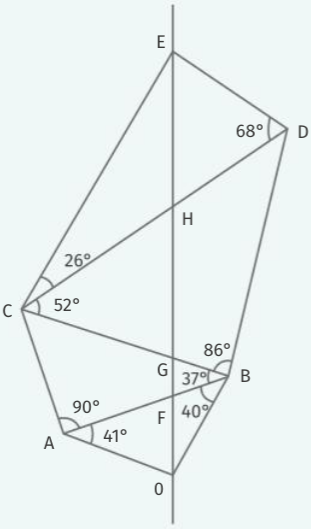
\includegraphics[scale=.65]{Ressources/1ES_C4_AE3_Fig4.png.png}

\begin{enumerate}
    \item Détermination du segment $OF$
        \begin{enumerate}
            \item Détermination des angles $\widehat{AOB}$ et $\widehat{AFO}$\\
            L'angle $\widehat{AOB}$ peut se calculer comme : $\widehat{AOB} = 180 - (40 + 41)$ = \SI{99}{\degree}.\\
            L'angle  $\widehat{AFO}$ peut se mesurer au rapporteur, il vaut \SI{70}{\degree}.
            \item Détermination de la longueur $OA$.\\
            La loi des sinus, dans le triangle $OAB$ donne : $$\dfrac{AB}{\sin{\widehat{AOB}}} = \dfrac{OB}{\sin{\widehat{OAB}}} = \dfrac{OA}{\sin{\widehat{OBA}}}$$
            $$OA = \dfrac{AB \times \sin{\widehat{OBA}}}{\sin{\widehat{AOB}}}$$
            $$OA = \dfrac{11 \times \sin{40}}{\sin{99}} = \SI{7,16}{km}$$
            \item Détermination de la longueur $OF$.\\
            La loi des sinus, dans le triangle $OAF$ donne : $$\dfrac{OA}{\sin{\widehat{OFA}}} = \dfrac{OF}{\sin{\widehat{OAF}}} = \dfrac{AF}{\sin{\widehat{AOF}}}$$
            $$OF = \dfrac{OA \times \sin{\widehat{OAF}}}{\sin{\widehat{OFA}}}$$
            $$OF = \dfrac{7,16 \times \sin{41}}{\sin{70}} = \SI{5,00}{km}$$
        \end{enumerate}
    \item Détermination du segment $FG$
        \begin{enumerate}
            \item Détermination de l'angle $\widehat{BFG}$\\
            L'angle $\widehat{BFG}$ peut se déterminer comme : $\widehat{BFG} = \widehat{OFA}$ = \SI{70}{\degree}.
            \item Calcul de la longueur $BF$\\
             La loi des sinus, dans le triangle $OAF$ donne : $$\dfrac{OA}{\sin{\widehat{OFA}}} = \dfrac{OF}{\sin{\widehat{OAF}}} = \dfrac{AF}{\sin{\widehat{AOF}}}$$
             $$AF = \dfrac{OA \times \sin{\widehat{AOF}}}{\sin{\widehat{OFA}}}$$
            $$AF = \dfrac{7,16 \times \sin{69}}{\sin{70}} = \SI{7,11}{km}$$
            La longueur $BF$ se calcule comme $BF=AB-AF$ soit $$BF=11-7,11=\SI{3,89}{km}$$
            \item Détermination de la longueur $FG$\\
            La loi des sinus, dans le triangle $BFG$ donne : $$\dfrac{BF}{\sin{\widehat{BGF}}} = \dfrac{FG}{\sin{\widehat{FBG}}} = \dfrac{BG}{\sin{\widehat{BFG}}}$$
            $$FG = \dfrac{BF \times \sin{\widehat{FBG}}}{\sin{\widehat{BGF}}}$$
            $$FG = \dfrac{3,89 \times \sin{37}}{\sin{73}} = \SI{2,45}{km}$$
        \end{enumerate}
    \item Détermination du segment $GH$
        \begin{enumerate}
            \item Détermination de l'angle $\widehat{CGH}$\\
            L'angle $\widehat{CGH}$ peut se déterminer comme : $\widehat{CGH} = \widehat{BGF}$ = \SI{73}{\degree}.
            \item Calcul de la longueur $BC$
             La loi des sinus, dans le triangle $ABC$ donne : $$\dfrac{AB}{\sin{\widehat{ACB}}} = \dfrac{BC}{\sin{\widehat{BAC}}}=\dfrac{AC}{\sin{\widehat{ABC}}}$$
             $$BC=\dfrac{AB \times \sin{\widehat{BAC}}}{\sin{\widehat{ACB}}}$$
             $$BC=\dfrac{11 \times \sin{90}}{\sin{53}}=\SI{13,77}{km}$$
            \item Calcul de la longueur $CG$\\
            La loi des sinus, dans le triangle $BFG$ donne : $$\dfrac{BF}{\sin{\widehat{BGF}}} = \dfrac{FG}{\sin{\widehat{FBG}}} = \dfrac{BG}{\sin{\widehat{BFG}}}$$
            $$BG = \dfrac{BF \times \sin{\widehat{BFG}}}{\sin{\widehat{BGF}}}$$
            $$BG = \dfrac{3,89 \times \sin{70}}{\sin{73}} = \SI{3,82}{km}$$
            La longueur $CG$ se calcule comme $CG=BC-BG$ soit $$CG = 13,77 - 3,82 = \SI{9,95}{km}$$
            \item Détermination de la longueur $GH$\\
            La loi des sinus, dans le triangle $CGH$ donne : $$\dfrac{CG}{\sin{\widehat{CHG}}}=\dfrac{GH}{\sin{\widehat{GCH}}}=\dfrac{CH}{\sin{\widehat{CGH}}}$$
            $$GH=\dfrac{CG\times \sin{\widehat{GCH}}}{\sin{\widehat{CHG}}}$$
            $$GH=\dfrac{9,95\times \sin{52}}{\sin{55}}=\SI{9,57}{km}$$
        \end{enumerate}
    \item Détermination du segment $HE$
        \begin{enumerate}
            \item Détermination de l'angle $\widehat{DHE}$\\
            L'angle $\widehat{DHE}$ peut se déterminer comme : $\widehat{DHE} = \widehat{CHG}$ = \SI{55}{\degree}.
            \item Détermination de la longueur $CD$\\
            La loi des sinus, dans le triangle $BCD$ donne : $$\dfrac{BC}{\sin{\widehat{BDC}}}=\dfrac{CD}{\sin{\widehat{CBD}}}=\dfrac{BD}{\sin{\widehat{BCD}}}$$
            $$CD = \dfrac{BC \times \sin{\widehat{CBD}}}{\sin{\widehat{BDC}}}$$
            $$CD = \dfrac{13,77 \times \sin{86}}{\sin{42}} = \SI{20,53}{km}$$
            \item Détermination de la longueur $CH$\\
            La loi des sinus, dans le triangle $CGH$ donne : $$\dfrac{CG}{\sin{\widehat{CHG}}}=\dfrac{GH}{\sin{\widehat{GCH}}}=\dfrac{CH}{\sin{\widehat{CGH}}}$$
            $$CH=\dfrac{CG\times \sin{\widehat{CGH}}}{\sin{\widehat{CHG}}}$$
            $$GH=\dfrac{9,95\times \sin{73}}{\sin{55}}=\SI{11,62}{km}$$
            \item Détermination de la longueur $DH$\\
            La longueur $DH$ se calcule comme $DH=CD-CH$ soit $$DH = 20,53 - 11,62 = \SI{8,91}{km}$$
            \item Détermination de la longueur $EH$\\
            La loi des sinus, dans le triangle $DEH$ donne : $$\dfrac{DH}{\sin{\widehat{DEH}}} = \dfrac{EH}{\sin{\widehat{EDH}}} =\dfrac{DE}{\sin{\widehat{DHE}}}$$
            $$EH = \dfrac{DH \times \sin{\widehat{EDH}}}{\sin{\widehat{DEH}}}$$
            $$EH = \dfrac{8,91 \times \sin{68}}{\sin{39}} = \SI{13,13}{km}$$
        \end{enumerate}
    \item Détermination de la distance $OE$
        $$OE = OF + FG + GH+ EH$$
        $$OE = 5,00 + 2,45 + 9,57 + 13,13 = \SI{30,15}{km}$$
\end{enumerate}
\end{multicols}
\end{document}
